%
% 
%
% Copyright (C) 1997-2004 by Dimitri van Heesch.
%
% Permission to use, copy, modify, and distribute this software and its
% documentation under the terms of the GNU General Public License is hereby 
% granted. No representations are made about the suitability of this software 
% for any purpose. It is provided "as is" without express or implied warranty.
% See the GNU General Public License for more details.
%
% Documents produced by Doxygen are derivative works derived from the
% input used in their production; they are not affected by this license.

\documentclass[a4paper]{article}
\usepackage{a4wide}
\usepackage{makeidx}
\usepackage{fancyhdr}
\usepackage{float}
\usepackage{graphicx}
\usepackage{epsf}
\usepackage{doxygen}
\usepackage{multicol}
\usepackage{times}
\usepackage{alltt}
\usepackage[pdftex,
            pagebackref=true,
            colorlinks=true,
            linkcolor=blue
           ]{hyperref}
\makeindex
\setcounter{tocdepth}{1}
\renewcommand{\footrulewidth}{0.4pt}
\begin{document}
\begin{titlepage}
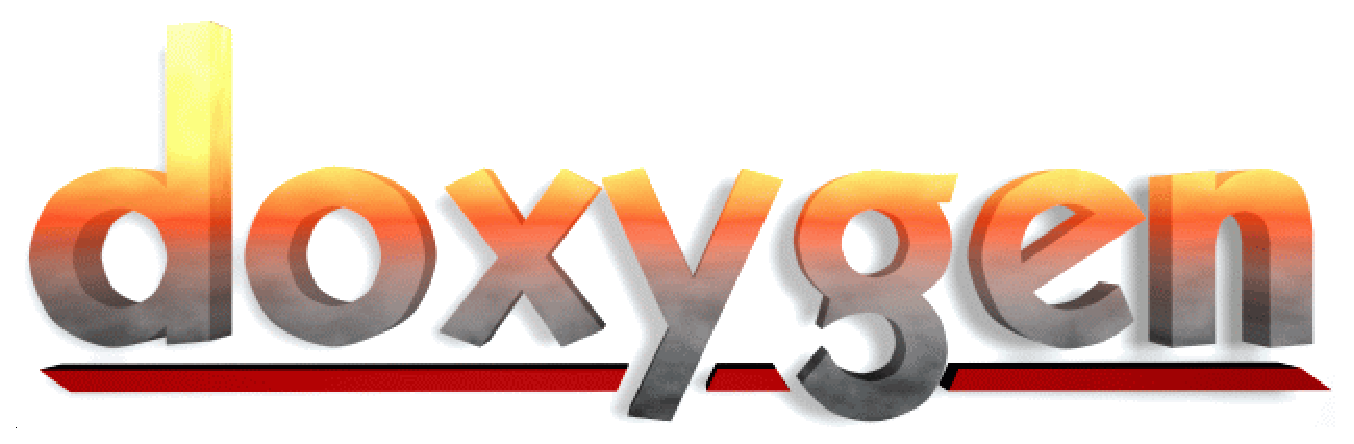
\includegraphics[width=\textwidth]{doxygen_logo}
\begin{center}
Manual for version $VERSION\\[2ex]
Written by Dimitri van Heesch\\[2ex]
\copyright 1997-2004
\end{center}
\end{titlepage}
\clearemptydoublepage
\tableofcontents
\clearemptydoublepage
\pagenumbering{arabic}
Bee\-Crypt started its life when the need for a portable and fast cryptography library arose at Virtual Unlimited in 1997. I'm still trying to make it faster, easier to use and more portable, in addition to providing better documentation.

Bee\-Crypt is released under the following license:

This library is free software; you can redistribute it and/or modify it under the terms of the GNU Lesser General Public License as published by the Free Software Foundation; either version 2.1 of the License, or (at your option) any later version.

This library is distributed in the hope that it will be useful, but WITHOUT ANY WARRANTY; without even the implied warranty of MERCHANTABILITY or FITNESS FOR A PARTICULAR PURPOSE. See the GNU Lesser General Public License for more details.

You should have received a copy of the GNU Lesser General Public License along with this library; if not, write to the Free Software Foundation, Inc., 59 Temple Place, Suite 330, Boston, MA 02111-1307 USA

Legal disclaimer: note that depending on where you are, the use of cryptography may be limited or forbidden by law. Before using this library, make sure you are legally entitled to do so.

Included in the library are: \begin{itemize}
\item entropy sources for initializing pseudo-random generators \item pseudo-random generators \begin{itemize}
\item FIPS-186 \end{itemize}
\item block ciphers \begin{itemize}
\item AES \item Blowfish \end{itemize}
\item hash functions \begin{itemize}
\item MD5 \item SHA-1 \item SHA-256 \end{itemize}
\item keyed hash functions (a.k.a. message authentication codes) \begin{itemize}
\item HMAC-MD5 \item HMAC-SHA-1 \item HMAC-SHA-256 \end{itemize}
\item multi-precision integer library, with assembler-optimized routines for a range of processors; optimized to perform well on both 32-bit and 64-bit machines \item probabilistic primality testing, with optimized small prime trial division \item discrete logarithm parameter generation over a prime field \item Diffie-Hellman key agreement \item DHAES encryption scheme \item DSA signature scheme \item El\-Gamal signature scheme (two variants) \item RSA keypair generation with chinese remainder theorem variables \item RSA public \& private key operations \end{itemize}


Planned for the future are: \begin{itemize}
\item compliance with and compliance statements for IEEE P1363 \item more blockciphers (Twofish, ... ) \item more blockcipher modes (OFB, ... ) \item more hash functions (RIPEMD-160, SHA-384, SHA-512, HAVAL, Tiger) \item RSA signatures as specified by RFC-2440. \item Elliptic Curves (ECDSA, ... ) \end{itemize}


The library has been tested on the following platforms: \begin{itemize}
\item Linux glibc 2.x alpha \item Linux glibc 2.x arm \item Linux glibc 2.x ia64 \item Linux glibc 2.x m68k \item Linux glibc 2.x ppc \item Linux glibc 2.x s390x \item Linux glibc 2.x sparc \item Linux glibc 2.x x86 \item Solaris 2.\mbox{[}6789\mbox{]} sparc (with Forte or GNU compilers) \item Solaris 2.\mbox{[}78\mbox{]} x86 (with Forte or GNU compilers) \item Tru64 Unix alpha \item Win32 (Windows 95, 98, NT 4.0, 2000, XP) \end{itemize}


The library is currently in the process of being ported to: \begin{itemize}
\item AIX (shared libraries don't seem to work in 64-bit mode) \item Darwin (javaglue doesn't compile yet) \item Cygwin (the DLL builds now, but needs to be tested) \end{itemize}


The structures in the library are geared towards exchange with Java and its security and cryptography classes. This library can also be accessed from Java by installing Bee\-Crypt for Java, a JCE 1.2 crypto provider and the counterpart of this library. 
\part{User Manual}
\input{install}
\input{starting}
\input{docblocks}
\input{lists}
\input{grouping}
\input{formulas}
PROJECT_NAME       = "Diagrams"
OUTPUT_DIRECTORY   = diagrams
HAVE_DOT           = YES
EXTRACT_ALL        = YES
GENERATE_LATEX     = NO
GENERATE_MAN       = NO
GENERATE_RTF       = NO
CASE_SENSE_NAMES = NO
ENABLE_PREPROCESSING       = YES
INPUT              = .
FILE_PATTERNS      = diagrams_*.h
QUIET              = YES
JAVADOC_AUTOBRIEF = YES

\input{preprocessing}
\input{external}
\input{faq}
\input{trouble}
\part{Reference Manual}
\input{features}
\input{history}
\input{doxygen_usage}
\input{doxytag_usage}
\input{doxywizard_usage}
\input{installdox_usage}
\input{output}
PROJECT_NAME     = "Automatic link generation"
OUTPUT_DIRECTORY = autolink
GENERATE_LATEX   = NO
GENERATE_MAN     = NO
GENERATE_RTF     = NO
CASE_SENSE_NAMES = NO
INPUT            = autolink.cpp
QUIET            = YES
JAVADOC_AUTOBRIEF = YES

\input{config}
\input{commands}
\input{htmlcmds}
\part{Developers Manual}
\input{arch}
\input{perlmod}
%\input{perlmod_tree}
\input{langhowto}
\printindex
\end{document}
